\section{Neuronales Netz}\label{sec:nn}
\subsection{Vorverarbeitung der Daten}
In der Analyse der Daten (siehe \autoref{sec:analyse}) wurde die Korrelation
der verschiedenen Eigenschaften von Wohnungen untersucht. Die dort gefundenen
Zusammenhänge können nun verwendet werden, um die Eingaben für das neuronale
Netz anzupassen. Dies ist notwendig, da ein neuronales Netz effizienter
die gewünschte Funktion erlernen kann, wenn bereits die Eingaben aussagekräftige
Informationen enthalten.

Aus diesem Grund werden für das Netz nicht einfach die in der Aufgabenstellung
gegebenen Attribute verwendet, sondern Attribute die eine hohe Korrelation besitzen
zusammengefasst und Attribute die einen geringen Einfluss auf die Bewertung haben
nicht verwendet.

Die folgende Auflistung zeigt die verwendeten Attribute:
\begin{itemize}\label{lst:Eigenschaften}
    \item \textbf{Kosten pro Quadratmeter (Miete, Quadratmeter):}
    \begin{itemize}
        \item löst die Korrelation zwischen Miete und der Anzahl der Quadratmeter und
        stellt so eine aussagekräftigere Eigenschaft für die Bewertung des Preis-Leistungsverhältnisses dar.
    \end{itemize}
    \item \textbf{Gesamtkosten (Nebenkosten, Miete, Kaution):}
    \begin{itemize}
        \item  fast alle Kosten zusammen. Dies ist möglich da diese Werte stark korrelieren.
    \end{itemize}
    \item \textbf{Kinderfreundlichkeit (Schule, Kindergarten):}
    \begin{itemize}
        \item beinhaltet die Nähe zur Schule und zum Kindergarten, wie in
        der Analyse der Korrelationsmatrix (siehe \autoref{sec:analyse}) entdeckt, haben diese beiden
        Merkmale einen entscheidenden Einfluss auf die Bewertung.
    \end{itemize}
    \item \textbf{Mobilität (Entfernung):}
    \begin{itemize}
        \item enthält das Entfernungsmerkmal. Die Korrelation zwischen Bewertung und Entfernung liefert eine schwache lineare
        Abhängigkeit. Die Notwendigkeit dieses Attributs könnte mit Hilfe eines Prototypen genauer überprüft werden.
    \end{itemize}
    \item \textbf{Ausstattung (Möbliert):}
    \begin{itemize}
        \item ist ein Attribut, welches aufgrund des Ergebnisses des Entscheidungsbaums
        mit in die Liste aufgenommen wird.
    \end{itemize}
    \item \textbf{Zimmerzahl}
    \begin{itemize}
        \item wird als Attribut hinzugenommen, da es eine lineare Abhängigkeit in der Korrelationsmatrix zeigt.
    \end{itemize}
\end{itemize}

Ausgeschlossene Attribute mit Korrelationswerten unter $0,1$ beziehungsweise $-0,1$ sind:\\
\emph{Stockwerk, Heizung, Hausmeister, S-Bahn, Alter, Aufzug, Lage, Küche, Bad, Balkon, Terrasse, Kehrwoche,}
und \emph{Garage}.\\

\paragraph{Umwandlung der Daten in numerische Werte}
Im nächsten Schritt müssen alle Werte in numerische Werte umgewandelt werden.
\begin{itemize}
    \item \textit{num-num} (z.B. 2-3 Zimmer):  Bei diesen Werten wird schlichtweg der Mittelwert gebildet.
    \item \textit{über/unter} (z.B. Alter über 100): Die Randwerte werden als tatsächliche Werte angesehen.
    \item \textit{nah/erreichbar/fern}: Hier bietet es sich an das Attribut als \textit{Entfernung zu ...} umzuschreiben.
                So kann für \textit{nah} der Minimalwert und für \textit{fern} der Maximalwert verwendet werden.
    \begin{itemize}
        \item nah: 0
        \item erreichbar: 0,5
        \item fern: 1
    \end{itemize}
    \item \textit{Boolean}: Für Werte, welche entweder erfüllt oder nicht erfüllt sind, wird 0 (nicht erfüllt) und 1 (erfüllt) verwendet.
\end{itemize}

Zusätzlich zur Umwandlung in numerische Werte müssen folgende Berechnungen durchgeführt werden:
\begin{equation}
        MieteProQuadratmeter = \frac{Miete}{Quadratmeter}
\end{equation}
\begin{equation}
    Gesamtkosten = Miete + Nebenkosten + Kaution
\end{equation}
\begin{equation}
    Kinderfreundlichkeit = \frac{Schule + Kindergarten}{2}
\end{equation}

\paragraph{Normierung der Daten}
Um eine Normierung der Daten durchzuführen müssen zunächst die Maximalwerte der
jeweiligen Attribute definiert werden. Die Werte werden anschließend auf Werte
zwischen 0 und 1 normiert. Dies ist notwendig, da eine Vorgewichtung der Attribute
vermieden werden soll.

\subsection{Netzstruktur}
Das Netz soll aus $6$ Eingabewerten einen Ausgabewert berechnen.
\autoref{fig:nnStruktur} zeigt die Struktur des Netzes zum Lösen
dieses Problems.
\begin{figure}[ht]
    \centering
    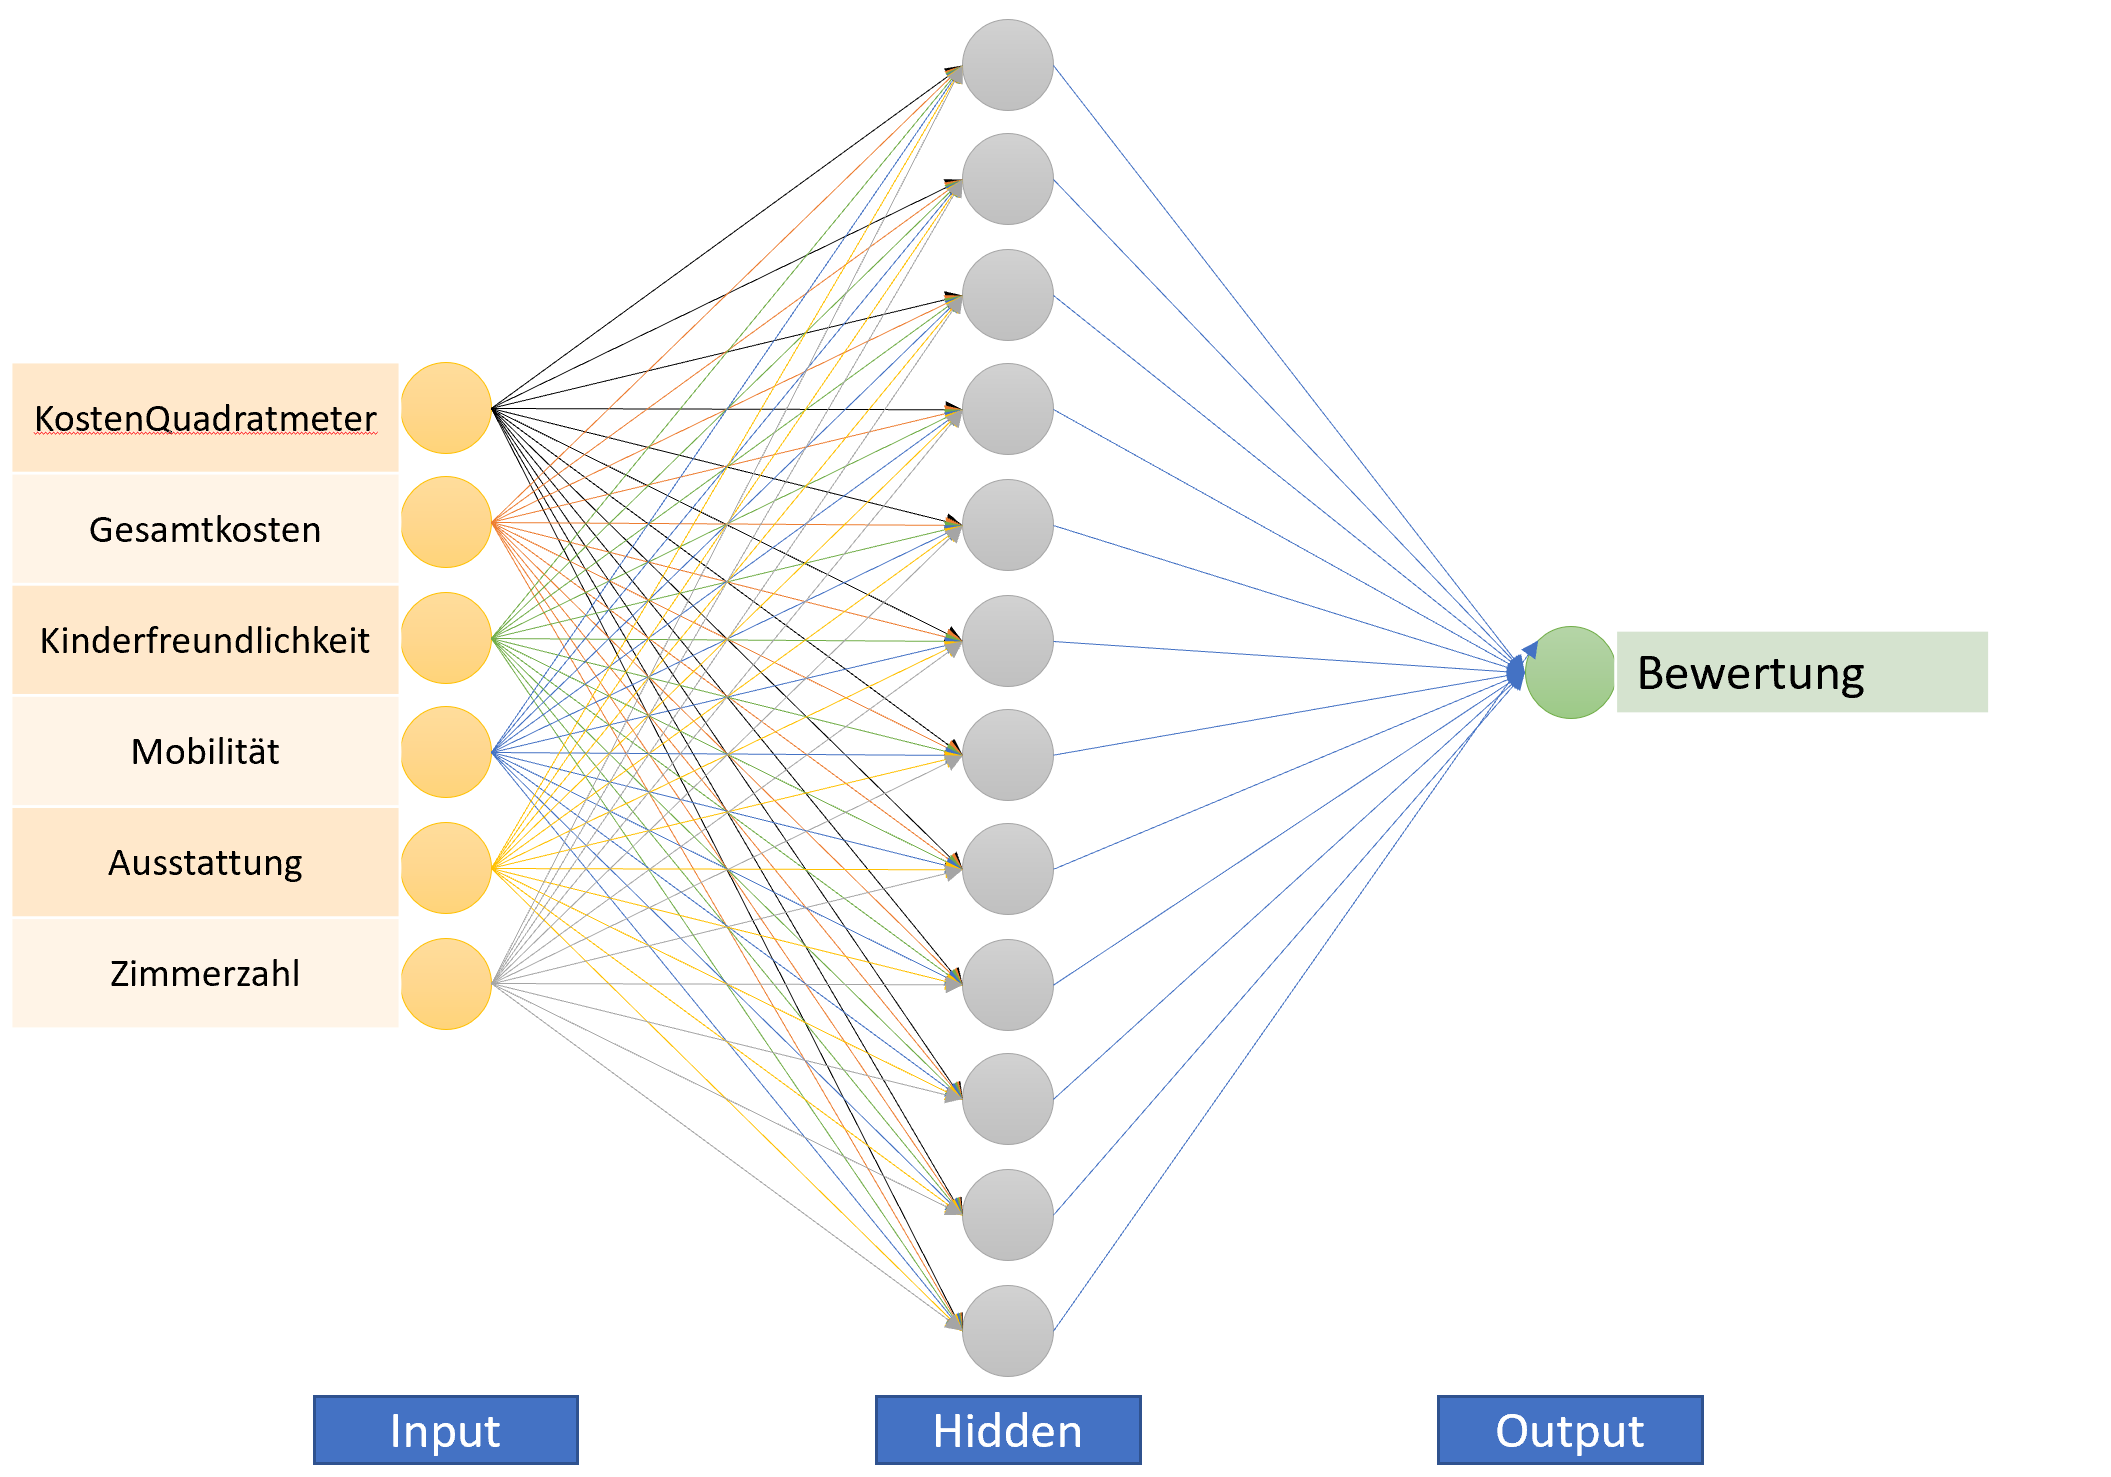
\includegraphics[width=15cm]{NNStruktur.PNG}
    \caption{Struktur des Neuronalen Netzes}
    \label{fig:nnStruktur}
\end{figure}

Die \textit{Input-Layer} besitzt $6$ Neuronen, dies entspricht der
Anzahl der Eigenschaften aus \autoref{lst:Eigenschaften}.
Die Anzahl der Neuronen in der \textit{Hidden-Layer} ergibt sich aus
$CountHidden = CountInput * 2$. Die \textit{Output-Layer} besitzt
lediglich ein Neuron, welches die Bewertung der Wohnung angibt.

\paragraph{Initiale Gewichtung der Neuronen}
Die initialen Gewichte für das Netz werden zufällig gesetzt. Diese werden in der Lernphase
mit Hilfe der Lernregel angepasst.

\paragraph{Aktivierungsfunktion und Schwellwert}
Die Aktivierungsfunktion eines Neurons gibt an, ab welchem Wert das Neuron das
einkommende Signal an die nächste Schicht weiterleitet.
Für diesen Anwendungsfall bietet sich eine Sigmoide-Funktion (\autoref{eqn:sigmoid}) an,
da diese die Eigenschaft besitzt ab dem Schwellwert allmählich
Signale weiterzuleiten.

Das bedeutet, ab einem Schwellwert von $0,5$, wird ein Signal weitergeleitet.
Allerdings erst bei einem Wert von $1$ ein maximales Signal.

\begin{equation}
    T_s(x) = \frac{1}{1+e^(\frac{x-S}{k})}
    \label{eqn:sigmoid}
\end{equation}

\paragraph{Lernregel}
Die Lernregel sorgt für die Anpassung der Gewichte. Das hier gewählte
Verfahren ist das \textit{Backpropagation-Verfahren}.
Es bietet sich an, da nach der Berechnung leicht der Netzfehler bestimmt werden kann.
Dieser Fehler wird anschließend zurück durch das Netz propagiert und die Gewichte
werden angepasst. Die Fehlerbestimmung erfolgt schichtweiße, beginnend mit der Output-Layer,
da hier der erwartete Wert zur Verfügung steht. Wurden die Fehler von jeder
Schicht bestimmt, werden die Gewichte angepasst.
Wie die Gewichte angepasst werden zeigt \autoref{eqn:gewichte}.
Hierbei wird das Gewicht des Neurons $j$ angepasst bei einer Eingabe,
von Neuron $i$. Der Fehler des aktuellen Neurons wird mit $\delta_j$ bezeichnet.
$x_i$ ist der Wert, welcher von $i$ an $j$ weitergegeben wird.
$\eta_i$ ist der Lernkoeffizient.
Dieser gibt an, wie stark die Gewichte angepasst werden und liegt zwischen 0 und 1.

\begin{equation}
    w_{ij}(t+1) = w_{ij}(t) + \eta * \delta_j*x_i
    \label{eqn:gewichte}
\end{equation}

Bei einfachen Problemen kann der Lernkoeffizent $=1$ sein.
Einerseits ist das hier beschriebene Problem nicht besonders einfach.
Andererseits sind nicht viele Schichten zur Lösung des Problems notwendig.
Daher bietet es sich an einen Lernkoeffizent von $0,7$ zu wählen.
Mit sinkendem Fehler kann dieser verringert werden,
um zu verhindern, dass die optimale Lösung \enquote{übersprungen} wird.

\subsection{Arbeitsweise/Ablauf}
Die folgende Auflistung zeigt, den Gesamtablauf des Netzes während eines
Lernschrittes.
\begin{enumerate}
    \item Initialisierung
    \item Berechnung der Aktivierung im \textit{Hidden-Layer}
    \item Berechnung Ausgabe der \textit{Hidden-Layer} mithilfe der Transferfunktion
    \item Berechnung Aktivierung im \textit{Output-Layer}
    \item Berechnung der Ausgabe durch die Transferfunktion.
    \item Berechnung des Fehlers der \textit{Output-Layer}
    \item Berechnung des Fehlers der \textit{Hidden-Layer}
    \item Berechnung des Fehlers der \textit{Input-Layer}
    \item Anpassung der Gewichte der \textit{Output-Layer}
    \item Anpassung der Gewichte der \textit{Hidden-Layer}
    \item Anpassung der Gewichte der \textit{Input-Layer}
\end{enumerate}